Due to the corona virus pandemic that started on March 2020, and has been ongoing since the beginning of this research project (June 2020 to August 2020), work had to be conducted remotely.

\section{Coding environment}

Due to the physical lab machines equipped with the GPUs being inaccessible during the pandemic, these machines had to be remotely accessed through SSH. As it is not efficient to implement an entire deep learning pipeline through a command line interface, a \textit{Jupyter Lab} session is created on a lab computer port and forwarded back to a local personal computer.\\

This is done by first logging onto the lab machine via SSH, activating the virtual environment and launching the Jupyter Lab session (these instructions are added into a bash script to be quickly executed):

\begin{lstlisting}
ssh agj6@agj6.host.cs.st-andrews.ac.uk -t ssh agj6@pc5-026-l.cs.st-andrews.ac.uk
source /cs/scratch/agj6/tf2/venv/bin/activate
cd ~/Projects/Breast-Cancer-Detection-and-Segmentation
jupyter lab --no-browser --port=8888
\end{lstlisting}

Keeping the first SSH session alive, a second terminal session is opened, and the port forwarding from the lab machine  to the personal computer is carried out using  the following command:

\begin{lstlisting}
nohup ssh -J agj6@agj6.host.cs.st-andrews.ac.uk agj6@pc5-026-l.cs.st-andrews.ac.uk -L 8888:localhost:8888 -N
\end{lstlisting}

To prevent the two SSH sessions from being automatically killed, some SSH settings are added to the ``\textit{/etc/ssh/ssh\_config}'' file, making the personal computer send a null packet to the lab machine every 5 minutes:

\begin{lstlisting}
Host *
    ServerAliveInterval 300
    ServerAliveCountMax 2
\end{lstlisting}

Finally, \url{http://localhost:8888}  is visited on a web browser to gain access to  the Jupyter Lab interface, containing a menu bar, a file explorer, code editor and command line for running python files (see Figure~\ref{fig:appendix-jupyter_interface}).

\begin{figure}[ht]
\centerline{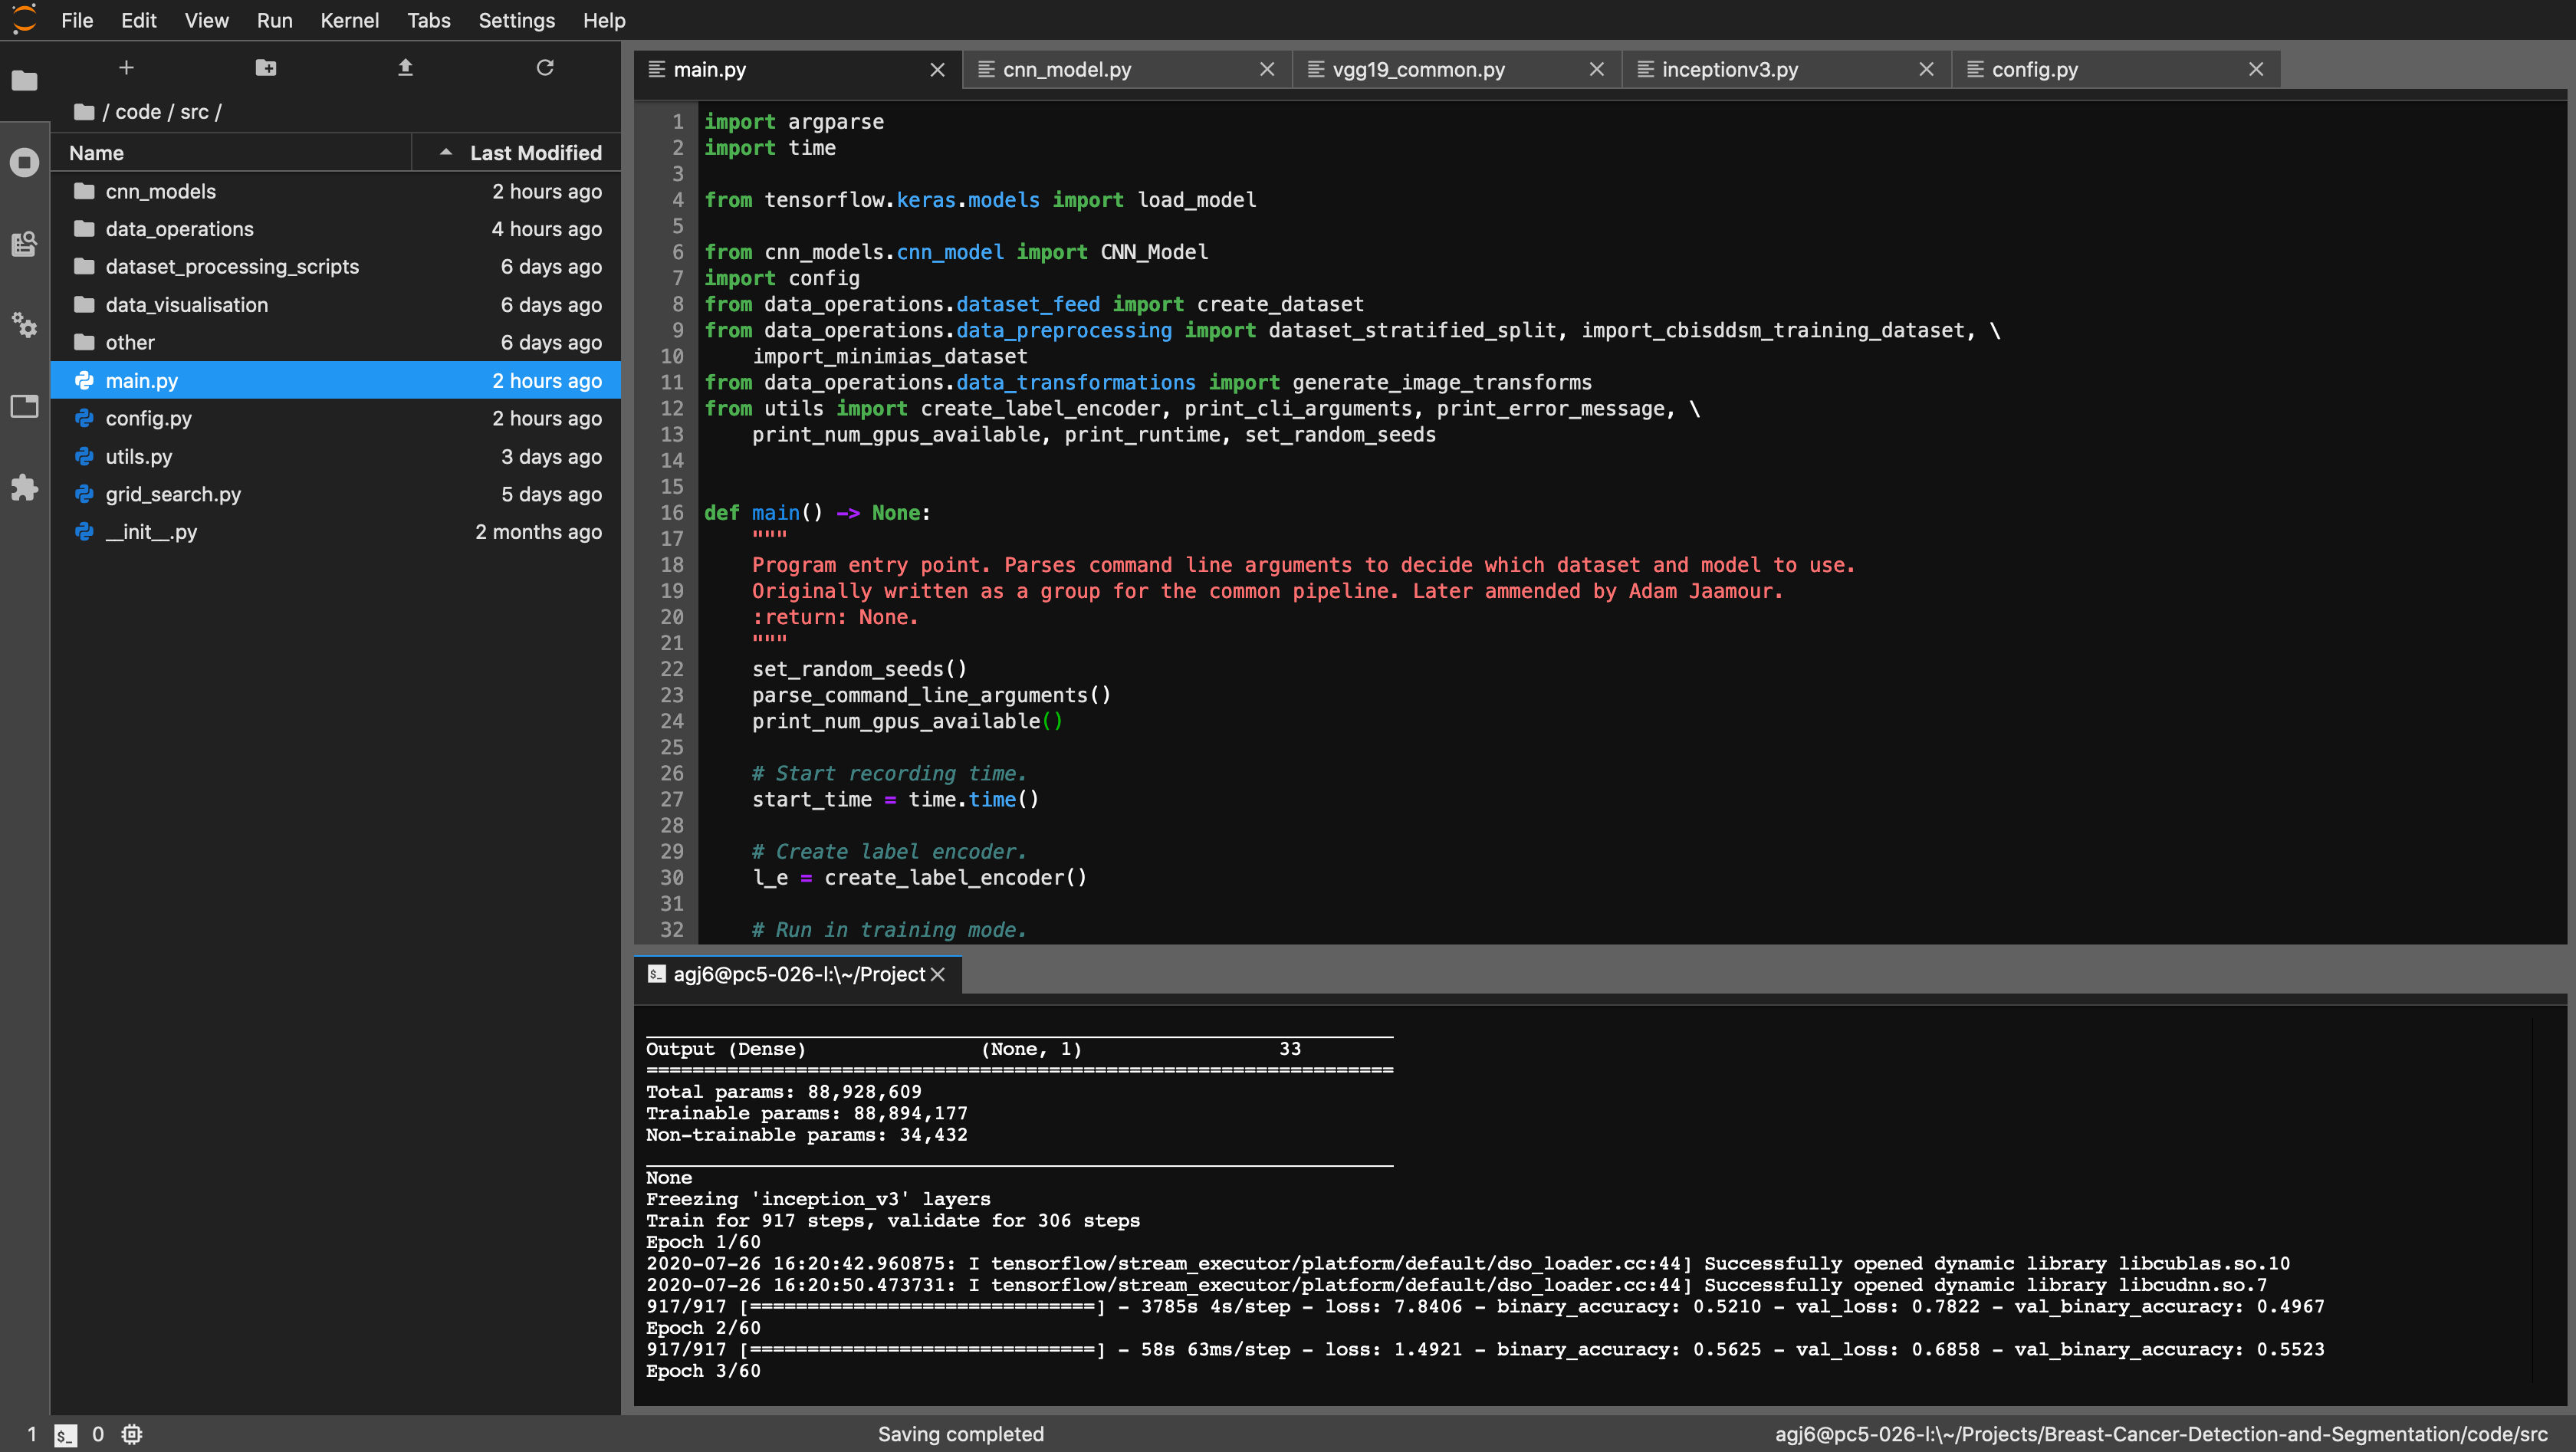
\includegraphics[width=\textwidth]{figures/appendix/jupyter_interface.png}}
\caption{\label{fig:appendix-jupyter_interface}Screenshot of the Jupyter Lab interface used to implement the project.}
\end{figure}

\section{Code collaboration}

For the group work part of the project, the code was collaboratively written and version controlled using GitHub, making use of the pull requests and merging features to combine code written by each group member. The code developed as a group can be found online at the following URL: \url{https://github.com/Adamouization/Breast-Cancer-Detection-Code}.

\section{Supervisor meetings}

Weekly video meetings with the project supervisor, Dr David Harris-Birtill, and the project co-supervisor, Lewis McMillan, were planned once per week via Microsoft Teams. Additional meetings with the other group members, Ashay Patel and Shuen-Jen Chen, were conducted via Microsoft Teams as well.